% Springer Nature journal template, version 3.1 (December 2024).
% Prepared for submission to General Relativity and Gravitation.
% Keep this manuscript, sn-jnl.cls, and both figure PDFs in one directory.
\documentclass[pdflatex,sn-mathphys-num]{sn-jnl}

\usepackage{graphicx}
\usepackage{amsmath,amssymb,amsfonts}
\usepackage{amsthm}
\usepackage{booktabs,tabularx,array}
\usepackage{float}
\usepackage{microtype}

\raggedbottom
\setlength{\emergencystretch}{3em}

\begin{document}

\title[KS--Schwarzschild surface-energy classification]{Surface-Energy Sign Classification for Timelike Kantowski--Sachs--Schwarzschild Junctions on the Ordinary Branch}

\author*[1]{\fnm{Ron} \sur{Bibb}}\email{ronbibb@gmail.com}
\affil*[1]{\orgname{Independent Researcher},
  \orgaddress{\city{Lilburn}, \state{Georgia}, \country{USA}}}

\abstract{We give a two-sector surface-energy classification for timelike spherical junctions between homogeneous Kantowski--Sachs (KS) geometry and the ordinary Schwarzschild branch. Every compatible finite-rapidity junction to the retained \(F(R)>0\) exterior has negative Israel surface density, so WEC and DEC fail independently of surface pressure; this ordering persists at \(F=0\), and sign indeterminacy begins strictly at \(F<0\). In the interior sector, retaining the increasing-\(R\) Schwarzschild side, we derive the exact positive-density interval and exhibit two distinct future-infalling local shell embeddings through the same bulk event, verified in ingoing Eddington--Finkelstein coordinates, with opposite density signs. For the positive-density witness, compatible acceleration data give \(p_s=\sigma/2\), so NEC, WEC, DEC, and the intrinsic \(2+1\)-dimensional SEC are all strictly satisfied. An invariant sufficient condition explains the exterior result: under the ordinary orientation, joining \((\nabla R)^2\le0\) to \((\nabla R)^2>0\) requires \(\sigma<0\), and KS geometry satisfies the first condition region-wide because its areal radius has no longitudinal spatial gradient. For an exact static comoving family, NEC fails precisely outside the Schwarzschild photon sphere, \(R_0=3m\). The combined causal-sector classification, exact interior interval, and regular-chart witnesses are the principal results.}

\keywords{junction conditions, thin shells, Kantowski--Sachs spacetime,
Schwarzschild spacetime, surface energy conditions}

\maketitle

\section{Introduction}

Matching spacetime regions across a hypersurface is a standard construction in gravitational physics. When the induced metric is continuous but the extrinsic curvature jumps, the jump is supported by a distributional surface stress tensor governed in general relativity by the Israel conditions \cite{ref1}. The method is used for stellar boundaries, collapsing shells, vacuum bubbles, wormholes, regular black holes, and proposed black-hole-to-cosmology transitions.


The last application requires careful causal and global bookkeeping. A transition surface may be timelike, spacelike, or null; the retained side of each geometry fixes the physically relevant normal orientations; and expansion of total spatial volume need not imply expansion of the areal radius. A Kantowski--Sachs representation does not by itself establish an expanding cosmology, and a Schwarzschild-time divergence at a horizon does not establish a reversed time direction.


Berezin, Kuzmin, and Tkachev (BKT) \cite{ref2} derive invariant outer-curvature and junction equations valid for arbitrary spherically symmetric shells, including dynamical geometries and changes between ordinary and wormhole branches. Farhi and Guth \cite{ref3}, Blau, Guendelman, and Guth \cite{ref4}, and Farhi, Guth, and Guven \cite{ref5} establish the closest physical lineage: the classical obstruction to producing an inflating universe on the ordinary asymptotic branch, the global dynamics of false-vacuum bubbles, and quantum access to the expanding wormhole-connected branch. Rosa and Carloni \cite{ref6} give a complementary covariant treatment for locally rotationally symmetric spacetimes and boundaries of all causal types. Here those tools yield a strict KS exterior theorem and, crucially, an exact constructive classification of the complementary interior sector. Sharif and Abbas \cite{ref18} previously calculated surface density and tangential pressure for a distinct Kantowski--Sachs--Minkowski shell, while Uzan, Ellis, and Larena \cite{ref19} matched static Kottler regions to a Kantowski--Sachs region at a cosmological horizon. Related work has used Kantowski--Sachs variables for distinct null-shell problems \cite{ref7}. Historic black-hole-to-cosmology constructions instead place the transition on a spacelike surface inside the black hole \cite{ref8,ref9}.


The same distinction is relevant to quantum-corrected black-hole interiors. Representative loop-quantum-gravity models treat the Schwarzschild interior as a homogeneous KS system: the classical singularity is replaced by a Nariai-type late-time region \cite{ref14}, a bounce into a white-hole interior \cite{ref15}, or a transition surface separating trapped and anti-trapped regions within a larger effective extension \cite{ref16}. An explicit Schwarzschild-to-KS construction using a localized layer instead places a spacelike S-brane inside the horizon \cite{ref17}. These models do not use the timelike ordinary-\(F>0\) junction studied in Theorem 1. The complementary calculation below explains the causal split: the strict negative-density ordering holds on the untrapped \(F>0\) side, whereas in the trapped \(F<0\) sector the sign becomes embedding-dependent and positive-density timelike data exist. This does not test the cited models' quantum dynamics or their spacelike transitions; it identifies the invariant boundary between the obstructed and sign-indefinite timelike sectors.


We first extract from BKT's invariant formula \cite[p.~2925, Eq.~(2.54a)]{ref2} a sufficient-condition proposition: if a spherical timelike shell joins a sector with \((\nabla R)^2\le0\) to an ordinary-oriented sector with \((\nabla R)^2>0\), the angular Israel jump is strictly positive and the surface density is negative. The KS product geometry then supplies a region-wide realization of the first hypothesis, while the retained Schwarzschild \(F>0\) exterior supplies the second. This makes the KS comparison strict at every matched radius: the magnitude of the KS angular curvature is smaller than the Schwarzschild contribution for either retained KS interval. Negative surface energy density is therefore universal within the theorem domain; NEC violation is a separate, stronger conclusion requiring additional trajectory data. Section 5.2 shows why FRW homogeneity does not imply the same result: its areal radius retains a longitudinal spatial gradient.


The principal result is the resulting causal-sector classification: a universal negative-density theorem for the retained \(F>0\) side and an exact sign criterion with both signs realized for \(F<0\). The derivation fixes the Schwarzschild orientation from the retained global region, obtains both independent mixed curvature components, closes the Israel and Codazzi relations, contrasts the KS product structure with FRW geometry, treats turning points without division by \(\dot R\), and verifies the interior witnesses in ingoing Eddington--Finkelstein coordinates.


Theorem 1 applies to the comoving interface and every compatible finite-rapidity shell embedding satisfying the proper-time and areal-matching relations while \(R>0\) and \(F>0\). Proposition 2 treats local future-infalling timelike segments with \(F<0\); it is not a global interior construction. Neither result covers spacelike transitions, alternative global gluings, finite-thickness layers, independent surface-spin sectors, or shell dynamics and stability.


One interpretive warning will matter later: Kantowski--Sachs total-volume expansion, governed by \(\Theta=H_A+2H_B\), does not imply expansion of the symmetry spheres, which requires \(H_B>0\). Section 9 gives the corresponding shear identity and explains why this distinction prevents the junction calculation from being read as evidence for an areal bounce.


\section{Geometry and conventions}

We use signature \((-+++)\). The Kantowski--Sachs metric is


\begin{equation}
ds_C^2=-N^2dt_C^2+A^2(t_C)d\chi^2+B^2(t_C)d\Omega_2^2.
\tag{1}
\end{equation}

After deriving the normalization condition we choose KS-side proper time \(N=1\), with


\begin{equation}
H_A=\frac{1}{A}\frac{dA}{dt_C},
\qquad
H_B=\frac{1}{B}\frac{dB}{dt_C},
\qquad
\Theta=H_A+2H_B.
\tag{2}
\end{equation}

The moving KS-side embedding is


\begin{equation}
X_C^\mu=(t_C(\tau),\chi(\tau),\theta,\phi),
\qquad
R(\tau)=B(t_C(\tau)).
\tag{3}
\end{equation}

The comoving case has \(\dot\chi=0\); the moving case permits every compatible finite-rapidity embedding satisfying Eq. (3), the proper-time normalizations, and the differentiated matching relation (18). Here finite rapidity means finite \(X=\sinh\zeta\), where \(\zeta\) is the shell's hyperbolic rapidity relative to the comoving KS frame; limiting sequences with \(X\to\infty\) are outside the theorem. Thus \(R(\tau)\), \(X(\tau)\), and their derivatives are not independent trajectory data once the bulk function \(B(t_C)\) and an embedding have been chosen. A dot denotes \(d/d\tau\), where \(\tau\) is shell proper time. Both embeddings are future oriented: we choose \(\dot t_C>0\), and in the \(F>0\) Schwarzschild region we choose \(\dot T>0\). Thus Eq. (15) uses the positive root \(\gamma=\dot t_C=\sqrt{1+X^2}\), while Eq. (10) uses \(\dot T=\beta/F>0\).


The Schwarzschild-side geometry is


\begin{equation}
ds_P^2=-F(R)dT^2+\frac{dR^2}{F(R)}+R^2d\Omega_2^2,
\qquad
F(R)=1-\frac{2m}{R},
\tag{4}
\end{equation}

where \(m=GM/c^2\). Its shell embedding is


\begin{equation}
X_P^\mu=(T(\tau),R(\tau),\theta,\phi).
\tag{5}
\end{equation}

The theorem concerns \(F(R)>0\). The limit \(F\to0^+\) is treated only as a chart-control limit.


The first junction condition is imposed explicitly. Pulling back either bulk metric to the shell gives the common induced metric \(ds_\Sigma^2=-d\tau^2+R^2(\tau)d\Omega_2^2\); equality of the angular components is precisely the areal matching relation \(R(\tau)=B(t_C(\tau))\) in Eq. (3). The temporal component is the proper-time normalization used below on each side.


The surface tensor is


\begin{equation}
\Sigma^a{}_b=\operatorname{diag}(-\sigma,p_s,p_s).
\tag{6}
\end{equation}

To fix the signed junction unambiguously, introduce a Gaussian-normal coordinate \(\eta\) in a neighborhood of the shell, with \(\eta=0\) on \(\Sigma\), \(\eta<0\) on the retained KS side, and \(\eta>0\) on the retained Schwarzschild side. We use the single normal


\[
n_\mu=\nabla_\mu\eta,
\]

directed from \(M_C\) to \(M_P\). The symbols \(n_{\mu,C}\) and \(n_{\mu,P}\) below are its one-sided limits, not two independently chosen outward normals. In particular, the common normal points out of the retained KS region and into the retained Schwarzschild exterior. We define


\begin{equation}
[K^a{}_b]=K^a{}_{b,P}-K^a{}_{b,C}
\tag{7}
\end{equation}

and use


\begin{equation}
[K_{ab}]-h_{ab}[K]
=-\frac{8\pi G}{c^4}\Sigma_{ab},
\qquad
K_{ab}=e_a{}^\mu e_b{}^\nu\nabla_\mu n_\nu.
\tag{8}
\end{equation}

The convention is anchored by \(K^\theta{}_\theta=+1/R\) for the outward normal to a round sphere in flat space. Orientation signs \(\epsilon_P,\epsilon_C\in\{-1,+1\}\) encode the components of this same common normal in the two coordinate charts.



\begin{table}[t]
\centering
\caption{Core conventions.}
\small
\begin{tabularx}{\textwidth}{@{}XX@{}}
\toprule
Object & Convention \\
\midrule
Metric signature & \((-+++ )\) \\
Jump & \([K^a{}_b]=K^a{}_{b,P}-K^a{}_{b,C}\) \\
Surface tensor & \(\Sigma^a{}_b=\mathrm{diag}(-\sigma,p_s,p_s)\) \\
Extrinsic curvature & \(K_{ab}=e_a{}^\mu e_b{}^\nu\nabla_\mu n_\nu\) \\
Common normal & \(n=d\eta\), directed from retained KS side to retained Schwarzschild side \\
Ordinary retained exterior & \(\epsilon_P=+1\) \\
Theorem domain & \(F(R)>0\), finite real \(X\) \\
\bottomrule
\end{tabularx}
\end{table}

Figure 1 summarizes the declared geometry, retained regions, and normal orientations.


\begin{figure}[t]
\centering

\includegraphics[width=0.72\textwidth]{figure1_junction_orientation.pdf}
\caption{Declared spherical timelike junction with the single Gaussian normal \(n=d\eta\) directed from \(M_C\) to \(M_P\). The retained Schwarzschild region contains spatial infinity, so the Schwarzschild-side limit of the common normal points toward increasing areal radius and \(\epsilon_P=+1\). On the KS side, retaining \(\chi\le\chi_\Sigma\) gives \(\epsilon_C=+1\), while retaining \(\chi\ge\chi_\Sigma\) gives \(\epsilon_C=-1\); in both cases the common normal points out of the retained KS region toward the Schwarzschild side. In both panels the retained KS region is drawn to the left of the shell, so the \(+\chi\) direction points page-right in Case A and page-left in Case B. The \(\epsilon_P=-1\) algebraic branch retains a different Schwarzschild side and is not a sign alternative for this gluing.}
\end{figure}

\section{Common-normal and retained-side lemma}

\textbf{Lemma 1.} Let \(n=d\eta\) be directed from the retained KS region to the retained Schwarzschild region. If the Schwarzschild side contains spatial infinity, then \(\epsilon_P=+1\). On the KS side, retaining \(\chi\le\chi_\Sigma\) gives \(\epsilon_C=+1\), while retaining \(\chi\ge\chi_\Sigma\) gives \(\epsilon_C=-1\). Thus


\begin{equation}
\epsilon_P=+1,
\qquad
\epsilon_C=
\begin{cases}
+1,&\chi\le\chi_\Sigma\ \text{retained},\\
-1,&\chi\ge\chi_\Sigma\ \text{retained}.
\end{cases}
\tag{9}
\end{equation}

\textbf{Proof.} The areal coordinate increases from the shell toward the asymptotically flat end. The Schwarzschild-side limit of the common normal derived below has \(n_P^R=\epsilon_P\beta\), with \(\beta>0\). Because increasing \(\eta\) enters the retained exterior, \(\epsilon_P=+1\). On the KS side, \(n_C^\chi=\epsilon_C\gamma/A\). If the retained interval is \(\chi\le\chi_\Sigma\), increasing \(\eta\) crosses its boundary toward increasing \(\chi\), so \(\epsilon_C=+1\). If the retained interval is \(\chi\ge\chi_\Sigma\), the crossing is toward decreasing \(\chi\), so \(\epsilon_C=-1\). \(\square\)


The algebraic branch \(\epsilon_P=-1\) retains the opposite side or describes a throat/back-to-back gluing; it is the branch used for wormhole-connected false-vacuum-bubble constructions \cite{ref4,ref5}. It is not an alternative convention for the same exterior. Reversing the single common normal while also reversing the jump order leaves the physical surface tensor unchanged.


The KS-side sign therefore labels two explicit retained-side gluings, not an independently adjustable normal: \(\epsilon_C=+1\) for \(\chi\le\chi_\Sigma\) retained and \(\epsilon_C=-1\) for \(\chi\ge\chi_\Sigma\) retained. In both constructions the normal is the same geometrical object, directed from KS to Schwarzschild, the jump order remains Schwarzschild minus KS, and \(\epsilon_P\) remains fixed by spatial infinity. Theorem 1 proves the same sign conclusion for either gluing.


\section{Complete extrinsic curvature}

\subsection{Schwarzschild side}

Proper-time normalization gives


\begin{equation}
F\dot T^2-\frac{\dot R^2}{F}=1.
\tag{10}
\end{equation}

Define


\begin{equation}
\beta=\sqrt{F+\dot R^2},
\qquad
\dot T=\frac{\beta}{F}.
\tag{11}
\end{equation}

An oriented unit normal covector is


\begin{equation}
n_{\mu,P}
=\epsilon_P\left(-\dot R,\frac{\beta}{F},0,0\right),
\tag{12}
\end{equation}

with \(n_P^R=\epsilon_P\beta\). Direct calculation gives


\begin{equation}
\boxed{
K^\tau{}_{\tau,P}
=\epsilon_P\frac{\ddot R+m/R^2}{\beta},
\qquad
K^\theta{}_{\theta,P}
=\epsilon_P\frac{\beta}{R}.
}
\tag{13}
\end{equation}

The acceleration form of \(K^\tau{}_{\tau,P}\) supplies its regular turning-point value without dividing by \(\dot R\).


\subsection{Moving Kantowski--Sachs side}

KS-side normalization is


\begin{equation}
\dot t_C^2-A^2\dot\chi^2=1.
\tag{14}
\end{equation}

Introduce


\begin{equation}
X=A\dot\chi,
\qquad
\gamma=\dot t_C=\sqrt{1+X^2}.
\tag{15}
\end{equation}

The oriented unit normal is


\begin{equation}
n_{\mu,C}
=\epsilon_C(-A\dot\chi,A\dot t_C,0,0).
\tag{16}
\end{equation}

Coordinate evaluation gives


\begin{equation}
\boxed{
K^\tau{}_{\tau,C}
=\epsilon_C\left(\frac{\dot X}{\gamma}+H_AX\right),
\qquad
K^\theta{}_{\theta,C}
=\epsilon_CXH_B.
}
\tag{17}
\end{equation}

Differentiating the areal matching condition yields


\begin{equation}
\frac{\dot R}{R}=\gamma H_B,
\tag{18}
\end{equation}

so


\begin{equation}
\boxed{
K^\theta{}_{\theta,C}
=\epsilon_C\frac{X\dot R}{\gamma R}.
}
\tag{19}
\end{equation}

An independent orthonormal-frame derivation uses


\begin{equation}
u^{\hat a}=(\gamma,X),
\qquad
n^{\hat a}=\epsilon_C(X,\gamma)
\tag{20}
\end{equation}

and reproduces both components exactly. In the comoving limit \(X=\dot X=0\), both KS-side components vanish.



\begin{table}[t]
\centering
\caption{Mixed extrinsic-curvature components.}
\small
\begin{tabularx}{\textwidth}{@{}XXX@{}}
\toprule
Side & \(K^\tau{}_\tau\) & \(K^\theta{}_\theta\) \\
\midrule
Schwarzschild side & \(\epsilon_P(\ddot R+m/R^2)/\beta\) & \(\epsilon_P\beta/R\) \\
Moving KS side & \(\epsilon_C(\dot X/\gamma+H_AX)\) & \(\epsilon_CXH_B=\epsilon_CX\dot R/(\gamma R)\) \\
Comoving KS side & \(0\) & \(0\) \\
\bottomrule
\end{tabularx}
\end{table}

\section{Thin-shell obstruction}

The invariant origin of the angular comparison is BKT's general formula \(K^\theta{}_\theta=R^{-1}n^\mu\nabla_\mu R\) and their angular Israel equation \cite[p.~2925, Eqs.~(2.54a) and (2.59a)]{ref2}. BKT's orientation sign records whether areal radius increases or decreases along the outward normal, the same geometric distinction encoded here by \(\epsilon_P\) and \(\epsilon_C\); our jump is ordered Schwarzschild minus KS as in Eq. (7), and Eq. (8) fixes the corresponding Israel sign.


\textbf{Proposition 1 (invariant sufficient condition).} Let a timelike spherical shell of areal radius \(R>0\) join two spherical regions, denoted \(C\) and \(P\), with one common normal directed from \(C\) to \(P\). Suppose that on the shell


\[
(\nabla R)^2_C\le0,
\qquad
(\nabla R)^2_P>0,
\]

and that the retained \(P\) region fixes the ordinary orientation \(K^\theta{}_{\theta,P}>0\). Then \(\Delta K_\theta>0\) and the angular Israel equation requires \(\sigma<0\), independently of the shell acceleration and surface pressure.


\textbf{Proof.} Decomposing the areal-radius gradient in the orthonormal tangent-normal plane of the shell gives, on either side,


\[
(\nabla R)^2=-\dot R^2+\left(RK^\theta{}_{\theta}\right)^2.
\]

The two invariant hypotheses and the ordinary orientation therefore imply


\[
\left|K^\theta{}_{\theta,C}\right|
\le\frac{|\dot R|}{R}
<\frac{\sqrt{\dot R^2+(\nabla R)^2_P}}{R}
=K^\theta{}_{\theta,P}.
\]

Thus \(\Delta K_\theta\ge K^\theta{}_{\theta,P}-|K^\theta{}_{\theta,C}|>0\), and Eq. (8) gives \(\sigma<0\). \(\square\)


Proposition 1 extracts the invariant sufficient condition used here. The following theorem shows that homogeneous KS geometry satisfies its interior hypothesis identically throughout the region and supplies the strict KS/ordinary-Schwarzschild realization with both retained-side gluings made explicit.


\textbf{Theorem 1 (KS ordinary-exterior specialization).} Consider a compatible finite-rapidity embedding (3) of a homogeneous Kantowski--Sachs region into a Schwarzschild exterior with \(R>0\) and \(F(R)>0\). Retain the Schwarzschild region containing spatial infinity, retain either \(\chi\le\chi_\Sigma\) or \(\chi\ge\chi_\Sigma\) on the KS side, and use the common-normal conventions (6)--(8). For every finite real \(X\) allowed by that embedding,


\begin{equation}
\Delta K_\theta
\equiv K^\theta{}_{\theta,P}-K^\theta{}_{\theta,C}>0
\tag{21}
\end{equation}

for either KS-side orientation. Consequently \(\sigma<0\) for every shell satisfying these hypotheses, independently of surface pressure and shell acceleration. This universal sign conclusion does not by itself imply \(\sigma+p_s<0\); NEC violation requires the additional condition \(\Delta K_\tau-\Delta K_\theta<0\).


\textbf{Proof.} Since \(\gamma=\sqrt{1+X^2}\),


\begin{equation}
\frac{|X|}{\gamma}<1.
\tag{22}
\end{equation}

Equation (19) therefore gives


\begin{equation}
\left|K^\theta{}_{\theta,C}\right|
<\frac{|\dot R|}{R}.
\tag{23}
\end{equation}

Because \(F>0\),


\begin{equation}
\frac{|\dot R|}{R}
<\frac{\sqrt{F+\dot R^2}}{R}
=\frac{\beta}{R}.
\tag{24}
\end{equation}

Lemma 1 fixes \(K^\theta{}_{\theta,P}=\beta/R>0\). Hence


\begin{equation}
\Delta K_\theta
\ge \frac{\beta}{R}
-\left|K^\theta{}_{\theta,C}\right|>0
\tag{25}
\end{equation}

for either \(\epsilon_C\). The Israel equation then gives


\begin{equation}
\boxed{
\sigma=-\frac{c^4}{4\pi G}\Delta K_\theta<0.
}
\tag{26}
\end{equation}

\(\square\)


\textbf{Remark 1 (ultrarelativistic limiting sequence).} The theorem concerns timelike shells and therefore finite rapidity. Along a sequence of compatible timelike embeddings with \(|X|\to\infty\), however, \(|X|/\gamma\to1\), and the limiting lower estimate remains


\[
\Delta K_\theta
\ge\frac{\sqrt{F+\dot R^2}-|\dot R|}{R}>0
\]

at every member with finite \(|\dot R|\) and \(F>0\). The gap need not be bounded uniformly away from zero when \(|\dot R|\) also grows without bound. This limiting observation does not add a null shell or an infinite-rapidity trajectory to the theorem's timelike domain.


\textbf{Corollary 1 (comoving interface).} In the comoving limit \(X=0\), the KS-side angular curvature vanishes and


\begin{equation}
\Delta K_\theta=\frac{\beta}{R}>0,
\qquad
\sigma<0.
\tag{27}
\end{equation}

Thus the ordinary-exterior obstruction includes the comoving interface as a strict special case.


\subsection{Invariant mass interpretation}

Proposition 1 already isolates the invariant mechanism; the coordinate proof of Theorem 1 remains decisive for the two explicit KS retained-side gluings because it fixes their signed Israel jumps. The same geometry also admits a useful region-wide interpretation through the Misner--Sharp geometrized mass length \(m_{\rm MS}=GM_{\rm MS}/c^2\), defined in spherical symmetry by


\begin{equation}
1-\frac{2m_{\rm MS}}{R}
=g^{\mu\nu}\nabla_\mu R\nabla_\nu R.
\tag{28}
\end{equation}

For any spherical timelike shell, decomposition of the areal-radius gradient into tangential and normal parts gives


\begin{equation}
g^{\mu\nu}\nabla_\mu R\nabla_\nu R
=-\dot R^2+\left(RK^\theta{}_{\theta}\right)^2.
\tag{29}
\end{equation}

On the Schwarzschild side, Eq. (28) gives \(m_{{\rm MS},P}=m\), and \(F>0\) is equivalent to \(2m/R<1\). On the homogeneous Kantowski--Sachs side, \(R=B(t_C)\) has no longitudinal spatial gradient. Consequently, throughout the KS region,


\begin{equation}
g_C^{\mu\nu}\nabla_\mu R\nabla_\nu R
=-\left(\frac{dB}{dt_C}\right)^2,
\tag{30}
\end{equation}

and therefore


\begin{equation}
\frac{2m_{{\rm MS},C}}{B}
=1+\left(\frac{dB}{dt_C}\right)^2\ge1,
\tag{31}
\end{equation}

with equality only where \(dB/dt_C=0\). This is a property of the KS region, independent of any shell embedding. On the shell, the areal matching relation gives


\begin{equation}
\left(\frac{dB}{dt_C}\right)^2
=\frac{\dot R^2}{\gamma^2}.
\tag{32}
\end{equation}

Thus the KS symmetry spheres are marginal, future trapped, or past trapped (anti-trapped), depending on the time orientation and the sign of \(dB/dt_C\). The retained \(F>0\) Schwarzschild exterior is untrapped. Their mass difference at the common areal radius is


\begin{equation}
\frac{2(m_{{\rm MS},C}-m_{{\rm MS},P})}{R}
=F+\frac{\dot R^2}{\gamma^2}>0.
\tag{33}
\end{equation}

Equations (28)--(33) give the physical content of Proposition 1 in the KS specialization: the shell joins a KS sector satisfying \(2m_{{\rm MS},C}/B\ge1\), whose spheres are trapped, anti-trapped, or marginal according to time orientation, to an ordinary untrapped exterior with smaller enclosed Schwarzschild mass length. The mass ordering alone does not determine the orientation sign of \(K^\theta{}_{\theta}\); the ordinary Schwarzschild-side orientation and the explicit retained-side construction are therefore essential to the signed conclusion. Proposition 1 makes BKT's invariant condition explicit, and Theorem 1 proves its strict KS/ordinary-exterior realization. The complementary \(F<0\) Schwarzschild region is trapped or anti-trapped, with the classification fixed by time orientation.


\subsection{Why homogeneity does not impose the same result in FRW}

The obstruction is not a consequence of spatial homogeneity alone. In a Friedmann--Robertson--Walker region,


\begin{equation}
ds^2=-dt^2+a^2(t)\left(\frac{dr^2}{1-kr^2}+r^2d\Omega_2^2\right),
\qquad R=a(t)r,
\tag{34}
\end{equation}

the areal radius has both temporal and radial gradients. Hence


\begin{equation}
g^{\mu\nu}\nabla_\mu R\nabla_\nu R
=-H^2R^2+1-kr^2,
\tag{35}
\end{equation}

and the positive radial term can make the symmetry spheres untrapped. The KS step in Eq. (30), where the longitudinal spatial derivative vanishes identically, therefore has no automatic FRW analogue. BKT's general treatment and FRW appendix contain the corresponding outer-curvature formulas \cite[pp.~2942--2943, Appendix B]{ref2}. The comparison identifies the KS geometric property that makes inequality (25) strict.


\subsection{Complementary interior sector: both density signs occur}

For a finite-rapidity timelike crossing of \(F=0\), the regular-chart relation requires \(\dot R\ne0\), and Eq. (25) survives as


\[
\left|K^\theta{}_{\theta,C}\right|<\frac{|\dot R|}{R}
=K^\theta{}_{\theta,P}.
\]

Thus \(\sigma<0\) still holds on the horizon itself. The horizon is the invariant boundary of the two classified open sectors, but sign indeterminacy begins strictly in \(F<0\).


\textbf{Lemma 2 (interior retained-side orientation).} Let a future-infalling timelike shell segment lie in Schwarzschild Kruskal region II, with \(F=-f<0\). Retain on the Schwarzschild side the connected increasing-\(R\) side whose closure meets the future horizon and continues into asymptotically flat region I. Direct the common normal from KS into that retained Schwarzschild side. Then \(\epsilon_P=+1\) and \(K^\theta{}_{\theta,P}=\beta/R>0\).


\textbf{Proof.} In ingoing Eddington--Finkelstein coordinates, a future-infalling timelike trajectory has \(\dot v=1/(\beta-\dot R)>0\). The common-normal construction gives \(n^R=\epsilon_P(-\dot R+F\dot v)=\epsilon_P\beta\). The retained side is the one reached in the increasing-\(R\) normal direction, so \(n^R>0\) and \(\epsilon_P=+1\). \(\square\)


With this orientation,


\[
K^\theta{}_{\theta,P}=\frac{\sqrt{\dot R^2-f}}{R}>0,
\qquad
\dot R^2>f,
\]

where the second inequality is the timelike-shell condition. The KS term remains


\[
K^\theta{}_{\theta,C}
=\epsilon_C\frac{X\dot R}{\gamma R}.
\]

If \(\epsilon_CX\dot R\le0\), then \(\Delta K_\theta>0\) and \(\sigma<0\). If the KS term is aligned positively with the Schwarzschild term, \(\epsilon_CX\dot R>0\), then \(\sigma>0\) precisely when


\[
\frac{X^2\dot R^2}{1+X^2}>\dot R^2-f.
\]

Equivalently, the positive-density interval is


\[
\boxed{
f<\dot R^2<(1+X^2)f,
\qquad
\epsilon_CX\dot R>0.
}
\]

Equality at the upper endpoint gives \(\sigma=0\). Outside this aligned interval, the surface density is negative. In invariant terms, when both angular curvatures are positively aligned, \(\sigma>0\) occurs when \((\nabla R)^2_C>(\nabla R)^2_P=F\); unlike Proposition 1, neither side is untrapped and no universal magnitude ordering remains.


\textbf{Proposition 2 (interior sign indeterminacy).} For a future-infalling timelike KS/Schwarzschild junction segment with \(F<0\), \(\epsilon_P=+1\), the retained Schwarzschild side extending toward increasing \(R\), and either explicitly fixed KS retained interval, the Israel surface density is not sign-definite. The aligned interval above is nonempty for every \(X\ne0\), and compatible local data exist with \(\sigma>0\). Two distinct local shell embeddings through the same bulk event, with the same retained-side signs but opposite longitudinal KS motion, can realize opposite density signs. They are not two states along one fixed shell trajectory.


\textbf{Proof by explicit paired witness.} Work in units where the matched radius is \(R=1\), and choose


\[
F=-\frac12,
\qquad
m=\frac34,
\qquad
\dot R=-2,
\qquad
\epsilon_P=+1,
\qquad
\epsilon_C=-1.
\]

For \(X=3\), one has \(\gamma=\sqrt{10}\), \(dB/dt_C=-2/\sqrt{10}\), and


\[
K^\theta{}_{\theta,P}=\frac{\sqrt{14}}2,
\qquad
K^\theta{}_{\theta,C}=\frac{3\sqrt{10}}5.
\]

Therefore


\[
\Delta K_\theta
=\frac{\sqrt{14}}2-\frac{3\sqrt{10}}5<0,
\qquad
\sigma>0.
\]

The corresponding Misner--Sharp ratios are


\[
\frac{2m_{{\rm MS},C}}{B}
=1-(\nabla R)^2_C
=\frac75,
\qquad
\frac{2m_{{\rm MS},P}}{R}
=1-F
=\frac32.
\]

Thus \(m_{{\rm MS},C}<m_{{\rm MS},P}\), reversing the exterior mass ordering in Eq. (33). This supplies the same invariant interpretation on both sides of the causal split.


In ingoing Eddington--Finkelstein coordinates, the future root and outward radial normal component are


\[
\dot v=\frac{1}{\beta-\dot R}=4-\sqrt{14}>0,
\qquad
n^R=-\dot R+F\dot v=\frac{\sqrt{14}}2>0.
\]

They satisfy \(-F\dot v^2+2\dot v\dot R=-1\), so the witness is a future-infalling timelike segment in a regular chart. Now reverse only the longitudinal motion, \(X=-3\). The proper-time factor, \(\dot R\), \(dB/dt_C\), both invariant gradient norms, the bulk event, and the retained-side signs are unchanged, while


\[
K^\theta{}_{\theta,C}=-\frac{3\sqrt{10}}5,
\qquad
\Delta K_\theta
=\frac{\sqrt{14}}2+\frac{3\sqrt{10}}5>0,
\qquad
\sigma<0.
\]

Thus both signs occur within the same local causal sector and retained-side gluing, on two distinct compatible local embeddings through the event. \(\square\)


The pair is not generated by a retained-region-preserving KS isometry. The reflection \(\chi-\chi_\Sigma\mapsto-(\chi-\chi_\Sigma)\) sends \(X\mapsto-X\) but also swaps \(\chi\le\chi_\Sigma\) with \(\chi\ge\chi_\Sigma\), and hence sends \(\epsilon_C\mapsto-\epsilon_C\). The product \(\epsilon_CX\), and therefore \(K^\theta{}_{\theta,C}\), is unchanged under the full reflected gluing. Proposition 2 instead holds \(\epsilon_C=-1\) and the retained interval fixed while reversing \(X\), so its two witnesses are not related by that isometry.


\textbf{Corollary 2 (energy-condition-satisfying interior witness).} The positive-density witness in Proposition 2 admits compatible local acceleration data for which NEC, WEC, DEC, and the intrinsic \(2+1\)-dimensional SEC all hold.


\textbf{Proof.} Retain the Proposition 2 data and choose


\[
\ddot R
=2a\beta-\frac{m}{R^2}
=\frac{6\sqrt{35}}5-\frac{31}{4},
\qquad
H_A=0,
\qquad
\dot X=0,
\qquad
\frac{d^2B}{dt_C^2}
=\frac{3\sqrt{35}}{25}-\frac{31}{40}.
\]

Because \(\gamma^2=10\), the differentiated matching relation closes exactly:


\[
\ddot R
=\gamma^2\frac{d^2B}{dt_C^2}
=\frac{6\sqrt{35}}5-\frac{31}{4}.
\]

Equation (17) gives \(K^\tau{}_{\tau,C}=0\), while Eq. (13) gives \(K^\tau{}_{\tau,P}=2a\). Hence \(\Delta K_\tau=2a\), where


\[
a\equiv-\Delta K_\theta
=\frac{3\sqrt{10}}5-\frac{\sqrt{14}}2>0.
\]

The Israel tensor is


\[
\sigma=\frac{c^4}{4\pi G}a>0,
\qquad
p_s=\frac{c^4}{8\pi G}a=\frac{\sigma}{2}>0.
\]

Consequently \(\sigma+p_s=3\sigma/2>0\), \(\sigma-|p_s|=\sigma/2>0\), and \(p_s=\sigma/2>0\). By the intrinsic criteria stated in Section 6, NEC, WEC, DEC, and the \(2+1\)-dimensional shell SEC are all strictly satisfied. \(\square\)


The compatible KS bulk data also have a positive energy density and satisfy the longitudinal bulk NEC. At the matched event, \(B=1\), \(H_A=0\), \(H_B=-2/\sqrt{10}\), and the chosen \(d^2B/dt_C^2\) give


\[
\kappa\rho=\frac75>0,
\qquad
\kappa(\rho+p_\chi)
=\frac{31}{20}-\frac{6\sqrt{35}}{25}>0.
\]

The transverse combination \(\rho+p_\perp\) depends on the otherwise free local acceleration \(dH_A/dt_C\), so no full bulk-NEC claim is made without specifying that datum.


Proposition 2 and Corollary 2 are local existence results, not a shell equation of motion or a global black-hole-to-cosmology construction. The asymmetry with Theorem 1 is intentional: a universal exterior obstruction requires a sign theorem for every compatible embedding, whereas interior sign indefiniteness and ordinary-matter admissibility require only explicit compatible witnesses. The corollary does not establish an equation of state, stability, or continuation, and it does not convert the timelike witness into the spacelike transition layers used in Refs. \cite{ref8,ref9,ref17}. It shows instead that those interior architectures lie on the side of the invariant boundary where the exterior negative-density theorem no longer applies.


\section{Surface tensor and energy conditions}

Define


\begin{equation}
\Delta K_\tau
=K^\tau{}_{\tau,P}-K^\tau{}_{\tau,C}.
\tag{36}
\end{equation}

The complete mixed Israel solution is


\begin{equation}
\boxed{
\sigma=-\frac{c^4}{4\pi G}\Delta K_\theta,
\qquad
p_s=\frac{c^4}{8\pi G}
\left(\Delta K_\tau+\Delta K_\theta\right).
}
\tag{37}
\end{equation}

All independent tensor residuals vanish after substitution. Useful combinations are


\begin{equation}
\sigma+p_s
=\frac{c^4}{8\pi G}
\left(\Delta K_\tau-\Delta K_\theta\right),
\tag{38}
\end{equation}

\begin{equation}
\sigma+2p_s
=\frac{c^4}{4\pi G}\Delta K_\tau.
\tag{39}
\end{equation}

\subsection{Null-energy criterion and a static comoving junction family}

The shell NEC is controlled by the signed scalar


\begin{equation}
\begin{aligned}
\mathcal N
&\equiv \Delta K_\tau-\Delta K_\theta \\
&=\frac{R\ddot R-\dot R^2-1+3m/R}{\beta R}
-\epsilon_C\left(
\frac{\dot X}{\gamma}+H_AX
-\frac{X\dot R}{\gamma R}
\right).
\end{aligned}
\tag{40}
\end{equation}

Equation (38) shows that the NEC is satisfied when \(\mathcal N\ge0\) and violated when \(\mathcal N<0\). The logical hierarchy is therefore sharp: \(\sigma<0\) is universal under Theorem 1, whereas NEC violation is not. The sign of \(\mathcal N\) depends additionally on the shell trajectory, acceleration, and KS-side kinematics and orientation.


\textbf{Proposition 3 (static comoving junction family).} Fix \(m>0\) and \(R_0>2m\). Suppose the declared junction contains an exact static comoving boundary segment on which


\[
X=\dot X=0,
\qquad
R(\tau)=B(t_C(\tau))=R_0,
\qquad
\dot R=\ddot R=0.
\]

Then the surface tensor is given by Eq. (41b). Its NEC and \(2+1\)-dimensional SEC are satisfied for \(2m<R_0<3m\), saturated at \(R_0=3m\), and violated for \(R_0>3m\). WEC and DEC fail throughout the family.


\textbf{Proof.} This hypothesis is stronger than an instantaneous turning point: \(B\) is constant along an open segment of the comoving boundary. Both KS-side extrinsic-curvature components vanish, whereas the ordinary-exterior Schwarzschild components remain nonzero. Equation (40) gives


\begin{equation}
\mathcal N_{\rm static}
=\frac{3m-R_0}{R_0^2\sqrt{F_0}},
\qquad
F_0=1-\frac{2m}{R_0}.
\tag{41a}
\end{equation}

The complete surface stress tensor for this family is


\begin{equation}
\sigma_0
=-\frac{c^4}{4\pi G}\frac{\sqrt{F_0}}{R_0},
\qquad
p_{s0}
=\frac{c^4}{8\pi G}
\frac{R_0-m}{R_0^2\sqrt{F_0}},
\qquad
w_s\equiv\frac{p_{s0}}{\sigma_0}
=-\frac{R_0-m}{2(R_0-2m)}.
\tag{41b}
\end{equation}

Consequently,


\begin{equation}
\sigma_0+p_{s0}
=\frac{c^4}{8\pi G}
\frac{3m-R_0}{R_0^2\sqrt{F_0}},
\qquad
\sigma_0+2p_{s0}
=\frac{c^4}{4\pi G}
\frac{m}{R_0^2\sqrt{F_0}}>0.
\tag{41c}
\end{equation}

Within the theorem domain, the shell NEC is therefore violated for \(R_0>3m\), saturated at \(R_0=3m\), and satisfied for \(2m<R_0<3m\).


Equivalently, \(-1<w_s<-1/2\) in the NEC-violating interval, \(w_s=-1\) at the threshold, and \(w_s<-1\) below it. These ratios classify the surface tensor algebraically; because \(\sigma_0<0\), they should not be read as ordinary positive-density fluid equations of state. For the intrinsic \(2+1\)-dimensional shell, the SEC requires NEC together with \(p_s\ge0\) \cite{ref20}. Equation (41b) shows \(p_{s0}>0\) throughout \(R_0>2m\), so the static family's SEC disposition is controlled entirely by the NEC. This proves the proposition. \(\square\)


The threshold \(R_0=3m\) is the Schwarzschild photon-sphere radius, so the required surface tensor violates NEC precisely outside the photon sphere within this static junction family. Define the dimensionless stresses


\[
\widetilde{\sigma}_0=\frac{8\pi Gm}{c^4}\sigma_0,
\qquad
\widetilde{p}_{s0}=\frac{8\pi Gm}{c^4}p_{s0}.
\]

Figure 2 displays these scaled quantities and the intrinsic NEC combination across the family. The same algebraic boundary appears in the distinct construction of a static Schwarzschild thin-shell wormhole, for which NEC is satisfied at the throat when \(2m<a_0\le3m\) \cite[Appendix A]{ref13}. That construction glues two Schwarzschild exteriors with wormhole orientations; Proposition 3 instead has vanishing KS-side curvature from a product region and retains one ordinary exterior. The shared threshold comes from the static Schwarzschild curvature combination.


\begin{figure}[t]
\centering
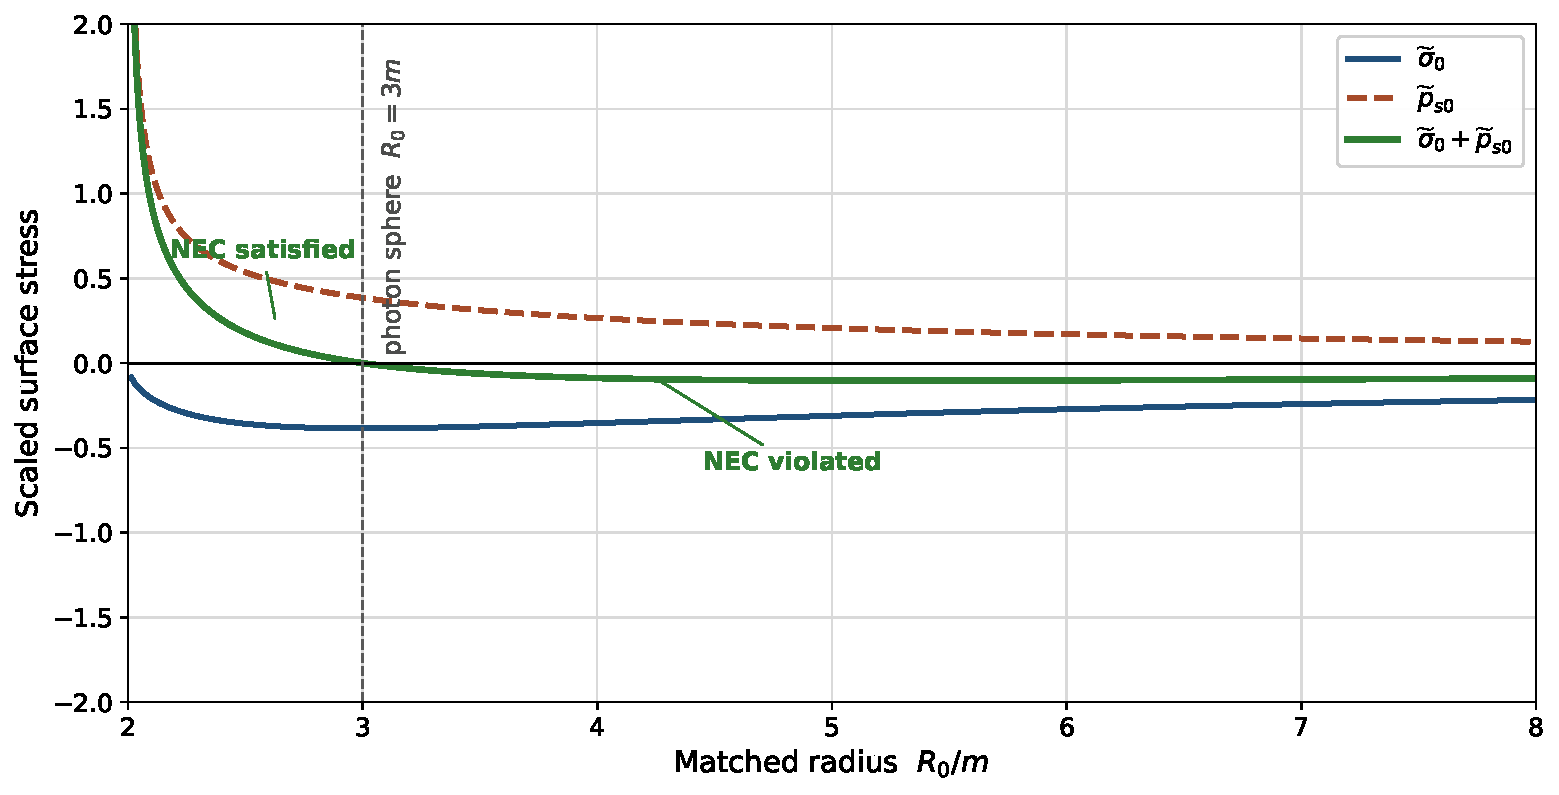
\includegraphics[width=0.82\textwidth]{figure2_static_family.pdf}
\caption{Scaled surface stresses \(\widetilde{\sigma}_0\) and \(\widetilde{p}_{s0}\), defined immediately above, for the exact static comoving junction configurations. Each plotted radius corresponds to a different Nariai scale \(\Lambda=R_0^{-2}\), not to a sequence of equilibria in one fixed bulk theory. The surface density remains negative, while the intrinsic NEC combination \(\widetilde{\sigma}_0+\widetilde{p}_{s0}\) changes sign at the Schwarzschild photon sphere, \(R_0=3m\). The intrinsic \(2+1\)-dimensional SEC additionally requires \(\widetilde p_{s0}\ge0\), which holds throughout this family. The plotting window truncates the pressure divergences as \(R_0\to2m^+\).}
\end{figure}

The family admits an explicit local isotropic bulk realization obtained by taking \(B=R_0\) throughout a KS interval. In \(c=1\) units, the independent Einstein equations then reduce to


\begin{equation}
\kappa\rho=\frac{1}{R_0^2},
\qquad
\kappa p_\chi=-\frac{1}{R_0^2},
\qquad
\kappa p_\perp=-\frac{\ddot A}{A}.
\tag{41d}
\end{equation}

Isotropy is therefore achieved with \(p_\chi=p_\perp=-\rho\) provided


\begin{equation}
\frac{\ddot A}{A}=\frac{1}{R_0^2},
\qquad
A(t_C)=A_+e^{t_C/R_0}+A_-e^{-t_C/R_0},
\tag{41e}
\end{equation}

on any interval where \(A>0\). This is the KS form of the Nariai \(dS_2\times S^2\) product region \cite{ref12}, with \(\Lambda=R_0^{-2}\). Its comoving boundary has zero KS-side extrinsic curvature and zero matter flux, so Eqs. (41b)--(41c) give the complete Israel layer required to attach it to a Schwarzschild exterior with vanishing cosmological constant. Each value of \(R_0\) fixes a different vacuum-energy scale; this is not a radius family within one theory with fixed \(\Lambda\). The scale-free statement belongs only to Theorem 1, whereas Proposition 3 is a special product solution with a radius-dependent bulk scale. This example is a static geometric junction witness: it establishes the local bulk geometry and required surface tensor, but supplies neither a surface action nor an equation of state proving dynamical support. It therefore does not establish equilibrium, radial stability, or a generic KS threshold.


At the level of thin-wall architecture, this realization parallels the false-vacuum interior/true-vacuum exterior problem studied by Blau, Guendelman, and Guth \cite{ref4}. The comparison is structural rather than an identification: their interior is four-dimensional de Sitter geometry and their analysis includes the ordinary and wormhole-connected global branches, whereas Proposition 3 uses a \(dS_2\times S^2\) product interior and isolates the ordinary-exterior static surface tensor. The photon-sphere threshold is therefore a result of this KS static specialization, not a critical radius imported from the de Sitter bubble problem.


More generally, Eqs. (41a)--(41c) give the required surface stress whenever the declared geometry contains an exact static comoving segment, without assuming this particular isotropic realization. They identify a nonempty, orientation-independent sector in which negative surface density is accompanied by \(\sigma+p_s<0\).


For the isotropic \(2+1\)-dimensional shell, WEC requires \(\sigma\ge0\) and \(\sigma+p_s\ge0\), while DEC requires \(\sigma\ge|p_s|\). Theorem 1 therefore proves failure of both WEC and DEC, regardless of \(p_s\). We use the intrinsic three-dimensional SEC,

\[
\left(\Sigma_{ab}-\Sigma h_{ab}\right)v^av^b\ge0
\]
for every timelike tangent vector \(v^a\), which for the type-I tensor (6) is equivalent to NEC together with \(p_s\ge0\) \cite[Proposition 3]{ref20}. In curvature variables these are \(\mathcal N\ge0\) and \(\Delta K_\tau+\Delta K_\theta\ge0\). Thus NEC and SEC remain trajectory-dependent in general, while Eq. (41a) gives an explicit NEC-violating subfamily.



\begin{table}[t]
\centering
\caption{Surface energy-condition disposition on the ordinary exterior branch.}
\small
\begin{tabularx}{\textwidth}{@{}XXX@{}}
\toprule
Condition & Requirement & Result from Theorem 1 \\
\midrule
NEC & \(\sigma+p_s\ge0\) & Trajectory-dependent; violated by the static comoving family for \(R_0>3m\) \\
WEC & \(\sigma\ge0\) and NEC & Violated because \(\sigma<0\) \\
DEC & \(\sigma\ge|p_s|\) & Violated because \(\sigma<0\) \\
SEC in \(2+1\) & NEC and \(p_s\ge0\) & Trajectory-dependent; for the static comoving family it fails exactly when \(R_0>3m\) \\
\bottomrule
\end{tabularx}
\end{table}

\section{Surface conservation}

The intrinsic shell metric is


\begin{equation}
ds_\Sigma^2=-d\tau^2+R^2(\tau)d\Omega_2^2.
\tag{42}
\end{equation}

Its surface divergence is


\begin{equation}
D_a\Sigma^a{}_\tau
=-\left[
\dot\sigma
+2\frac{\dot R}{R}(\sigma+p_s)
\right].
\tag{43}
\end{equation}

The factor of two is the area-expansion factor for the shell’s two angular directions. The distributional Bianchi identity requires


\begin{equation}
D_a\Sigma^a{}_b
+[T_{\mu\nu}n^\mu e^\nu{}_b]^P_C=0.
\tag{44}
\end{equation}

The Schwarzschild side is vacuum. For a comoving diagonal KS source


\[
T^{\hat a}{}_{\hat b}
=\operatorname{diag}(-\rho,p_\chi,p_\perp,p_\perp),
\]

only the longitudinal pressure enters the shell-crossing flux. Projection using the common normal gives


\begin{equation}
T_{\mu\nu,C}n_C^\mu e_\tau^\nu
=\epsilon_C\gamma X(\rho+p_\chi).
\tag{45}
\end{equation}

The Codazzi identity therefore reduces in \(c=1\) units to


\begin{equation}
\boxed{
\dot\sigma
+2\frac{\dot R}{R}(\sigma+p_s)
=-\epsilon_C\gamma X(\rho+p_\chi).
}
\tag{46}
\end{equation}

This is the general comoving diagonal-source conservation law needed for the theorem's KS class; it does not assume pressure isotropy. For the isotropic perfect-fluid specialization, \(p_\chi=p_\perp=p\), the KS-side energy and pressure equations are


\[
\kappa\rho=2H_AH_B+H_B^2+\frac{1}{B^2},
\qquad
\kappa p=-2\frac{dH_B}{dt_C}-3H_B^2-\frac{1}{B^2}.
\]

Their sum gives


\[
\frac{dH_B}{dt_C}-H_AH_B+H_B^2
=-\frac{\kappa}{2}(\rho+p).
\]

Using Eqs. (17)--(19), differentiating the Israel tensor and applying this identity reproduces Eq. (46) with \(p_\chi=p\), providing an independent closure check. The right-hand side is the kinematic flux measured when a moving shell crosses comoving KS matter; it is not a Schwarzschild-to-KS deposition law. In the comoving limit, \(X=0\) and the flux vanishes.


\section{Turning point and regular-chart controls}

At an exterior turning point, \(\dot R=0\). Equation (18) then implies \(H_B=0\), and


\begin{equation}
K^\theta{}_{\theta,C}=0,
\qquad
K^\theta{}_{\theta,P}
=\epsilon_P\frac{\sqrt F}{R}.
\tag{47}
\end{equation}

The ordinary branch retains \(\sigma<0\). The pressure remains finite for finite \(\ddot R,\dot X,H_A,\) and \(X\).


To control the Schwarzschild horizon coordinate singularity, introduce


\begin{equation}
v=T+r_*(R),
\qquad
\frac{dr_*}{dR}=\frac{1}{F}.
\tag{48}
\end{equation}

Then


\begin{equation}
ds_P^2=-F\,dv^2+2\,dv\,dR+R^2d\Omega_2^2.
\tag{49}
\end{equation}

Proper-time normalization gives


\begin{equation}
-F\dot v^2+2\dot v\dot R=-1,
\tag{50}
\end{equation}

with future-ingoing root


\begin{equation}
\dot v
=\frac{\beta+\dot R}{F}
=\frac{1}{\beta-\dot R}.
\tag{51}
\end{equation}

Using


\begin{equation}
n_{\mu,P}=\epsilon_P(-\dot R,\dot v,0,0),
\tag{52}
\end{equation}

direct calculation reproduces Eq. (13) exactly. For a genuinely infalling timelike shell with nonzero \(\dot R<0\), \(\beta\to-\dot R\) as \(F\to0^+\), so


\begin{equation}
\dot v\longrightarrow-\frac{1}{2\dot R},
\tag{53}
\end{equation}

which is finite. The surface tensor also remains finite for finite acceleration. This controls the \(F\to0^+\) limit of Theorem 1 and implies no reversed time direction. Proposition 2 separately treats local \(F<0\) timelike data directly in the same regular chart.


\section{Relation to prior work and limitations}

The affirmative result has two levels. Proposition 1 extracts an invariant sufficient condition: under the ordinary orientation, a timelike shell joining a sector with \((\nabla R)^2\le0\) to one with \((\nabla R)^2>0\) must carry negative surface density. Theorem 1 then supplies a geometric, region-wide realization. Because the Kantowski--Sachs product geometry has areal radius \(B(t_C)\) with no longitudinal spatial gradient, Eq. (31) shows that \(2m_{{\rm MS},C}/B\ge1\) identically throughout the region, with equality only where \(dB/dt_C=0\). The shell relation \(R=B\) is imposed only when evaluating a matched event. The obstruction therefore applies at every matched radius in the ordinary \(F>0\) exterior, with no critical radius or cosmological-constant scale.


BKT \cite{ref2} supply the general invariant angular-curvature formula and its surface-energy junction equation for arbitrary spherical shells, while Rosa and Carloni \cite{ref6} supply the encompassing covariant LRS framework. The new contribution is their combined causal-sector realization here: Proposition 1 states the invariant sufficient condition; Theorem 1 proves its strict, region-wide KS/ordinary-Schwarzschild form; and Proposition 2 derives the exact \(F<0\) positive-density interval and realizes both signs with regular future-infalling witnesses on one retained-side gluing. Sharif and Abbas \cite{ref18} instead study a KS--Minkowski shell, and Uzan, Ellis, and Larena \cite{ref19} match Kottler regions to KS at a cosmological horizon. The FRW comparison isolates the product-geometric premise of the KS theorem. The static \(3m\) NEC threshold also occurs in a Schwarzschild thin-shell wormhole \cite{ref13}; Proposition 3 contributes the KS/Nariai surface tensor and its interpretation rather than the radius alone.


The \(F=0\) horizon is the invariant boundary between the classified open sectors, not an arbitrary cutoff. The finite-rapidity timelike-crossing limit retains the strict negative-density ordering at \(F=0\); sign indeterminacy starts only at \(F<0\). There, Proposition 2 holds locally for \(\epsilon_P=+1\) and the increasing-\(R\) retained Schwarzschild side, and supplies two distinct embeddings with opposite density signs. Corollary 2 gives compatible local surface data satisfying all standard shell energy conditions. This does not establish a global interior gluing or the dynamics of the spacelike layers used in Refs. \cite{ref8,ref9,ref17}.


Proposition 1 is also distinct from the standard thin-shell-wormhole flare-out argument. A wormhole throat is a minimum of areal radius and uses outward normals on two back-to-back exterior copies, which fixes the angular-curvature signs through that global gluing. Here one common normal crosses two different regions, and the sufficient condition compares the causal character of their areal-radius gradients. Proposition 2 further shows that when both gradients are nonspacelike, reversing the longitudinal KS shell motion can reverse the density sign without changing the retained regions. The mechanisms are therefore related through the Israel angular equation but not identical.


The \(\epsilon_P=-1\) algebraic branch corresponds, after translating retained-region and normal conventions, to the wormhole-connected global constructions studied by Blau, Guendelman, and Guth and by Farhi, Guth, and Guven \cite{ref4,ref5}. Their false-vacuum result is dynamical and de Sitter-specific: the ordinary and wormhole branches determine whether an inflating bubble can expand into a child universe. The present classification instead follows from the KS product geometry and its missing longitudinal areal-radius gradient, giving a region-wide \(F>0\) sign theorem and a local \(F<0\) sign-indefinite complement. The BGG/FGG branch cannot therefore be treated as an algebraic sign alternative for the retained Schwarzschild side used here; it requires its own global regions and physical interpretation.


The Farhi--Guth past-incompleteness argument concerns the global causal structure and bulk energy conditions of inflating spacetimes \cite{ref3}. Determining its applicability to the Kantowski--Sachs interiors considered here is outside the present thin-shell analysis, which establishes only the sign of the distributional surface energy for the declared timelike matching.


Finally, negative \(\sigma\) is a distributional thin-shell result. A finite-thickness transition is the natural setting in which the obstruction could change or dissolve. A resolved layer may introduce anisotropic stress, spin transport, additional fields, or a varying embedding. Smoothing alone does not guarantee success: the integrated stress and conservation laws must still follow from a declared action.


The volume-versus-areal warning from the Introduction follows directly from the independent GR KS pressure equations \cite{ref11}. The same kinematical relations are recovered as the torsion-free limit of the Einstein--Cartan treatment in Ref. \cite{ref10}; no torsion or spin term is used here. In addition to the longitudinal equation displayed above, the angular equation is


\[
\kappa p=-\left(
\frac{dH_A}{dt_C}+\frac{dH_B}{dt_C}
+H_A^2+H_AH_B+H_B^2
\right).
\]

Subtracting the two pressure equations and defining \(s=H_A-H_B\) gives


\begin{equation}
\frac{ds}{dt_C}+\Theta s=\frac{1}{B^2}.
\tag{54}
\end{equation}

The symmetry-sphere curvature sources anisotropy, so \(\Theta>0\) does not imply \(H_B>0\). This kinematic implication is not part of Theorem 1, but it prevents the junction calculation from being reinterpreted as evidence for a bounce or child universe.


\section{Conclusions}

We obtained a surface-energy sign classification across the two Schwarzschild causal sectors. Under the ordinary orientation, a timelike spherical shell joining a sector with \((\nabla R)^2\le0\) to one with \((\nabla R)^2>0\) has a positive angular-curvature jump and hence \(\sigma<0\). The KS product geometry satisfies the first condition identically: \(2m_{{\rm MS},C}/B\ge1\) throughout the region. The retained Schwarzschild \(F>0\) side supplies the second condition, so Theorem 1 fixes the negative sign for either KS retained interval.


The finite-rapidity timelike-crossing limit remains negative-density at \(F=0\). In the complementary \(F<0\) sector, with \(\epsilon_P=+1\) and the increasing-\(R\) Schwarzschild side retained, no universal sign remains: positive density occurs for aligned KS angular curvature precisely when \(|F|<\dot R^2<(1+X^2)|F|\). Proposition 2 supplies two distinct future-infalling EF-regular local embeddings through the same bulk event, one with \(\sigma>0\) and the other with \(\sigma<0\). The positive witness reverses the exterior Misner--Sharp ordering, \(m_{{\rm MS},C}<m_{{\rm MS},P}\), and Corollary 2 supplies compatible acceleration data with \(p_s=\sigma/2\), so all intrinsic shell energy conditions hold strictly. This is a local geometric classification, not a dynamical or global transition construction.


Within the \(F>0\) theorem domain, WEC and DEC fail independently of surface pressure. NEC violation is not universal: it requires the additional trajectory condition \(\Delta K_\tau-\Delta K_\theta<0\). Proposition 3 proves that for the exact static comoving junction family this condition holds precisely outside the Schwarzschild photon sphere, \(R_0>3m\), with saturation at \(R_0=3m\); the \(2+1\)-dimensional SEC has the same threshold within that family. Its Nariai-type geometric witness has \(\Lambda=R_0^{-2}\), a scale specific to that auxiliary realization and absent from Theorem 1. The anisotropic-source surface conservation identity closes with longitudinal pressure \(p_\chi\), the turning-point limit preserves the exterior obstruction, and the curvature and orientation checks agree in Schwarzschild and ingoing Eddington--Finkelstein coordinates.


The result is a causal-sector classification for timelike thin shells: it identifies the invariant boundary at which the universal sign result ends and proves constructively that both density signs, including ordinary-matter surface data, occur on the interior side. Spacelike junctions, alternative global gluings, finite-thickness layers, and the dynamics and stability of the timelike witnesses remain outside its scope.


\section*{Acknowledgments}

This research was conducted independently, without institutional or grant support. R.B. thanks Hazel for her tireless support and patience throughout this research---and for saying yes on June 20th, in the middle of all of it.


Software used in this work includes Python, SymPy, SciPy, ReportLab, PGFPlots, and XeLaTeX.


\section*{Declarations}

\textbf{Funding:} None.


\textbf{Competing interests:} The author declares no competing interests.


\section*{Data and code availability}

No observational or experimental datasets were generated or analyzed in this study. The archived manuscript source, figure-generation scripts, symbolic and numerical verification suite, and exact pinned provenance modules are available through the stable Zenodo archive, doi:10.5281/zenodo.21872425. Development history remains available at https://github.com/RonBibb/junction-ec-paper.


\appendix
\section{Orthonormal-frame check}

In the KS-side \(t_C\)-\(\chi\) plane, use


\begin{equation}
u^{\hat a}=(\gamma,X),
\qquad
n^{\hat a}=\epsilon_C(X,\gamma).
\tag{A1}
\end{equation}

Writing \(X=\sinh\zeta\) and \(\gamma=\cosh\zeta\) gives \(\dot\zeta=\dot X/\gamma\). Normal projection of the shell acceleration yields


\begin{equation}
n_{\hat a}a^{\hat a}
=\epsilon_C\left(\frac{\dot X}{\gamma}+H_AX\right),
\tag{A2}
\end{equation}

which reproduces the temporal component in Eq. (17). Since \(B\) depends only on \(t_C\),


\begin{equation}
K^\theta{}_{\theta,C}
=\frac{1}{B}n^\mu\nabla_\mu B
=\epsilon_CXH_B,
\tag{A3}
\end{equation}

reproducing the angular component and providing a derivation independent of the coordinate calculation.


\section{Israel component algebra}

Spherical symmetry gives


\begin{equation}
[K^a{}_b]
=\operatorname{diag}(\Delta K_\tau,\Delta K_\theta,\Delta K_\theta),
\qquad
[K]=\Delta K_\tau+2\Delta K_\theta.
\tag{B1}
\end{equation}

The mixed \(\tau\)-component of Eq. (8) gives


\begin{equation}
-2\Delta K_\theta
=\frac{8\pi G}{c^4}\sigma,
\tag{B2}
\end{equation}

while either angular component gives


\begin{equation}
-\Delta K_\tau-\Delta K_\theta
=-\frac{8\pi G}{c^4}p_s.
\tag{B3}
\end{equation}

These are Eq. (37). Substitution into all three mixed equations gives zero residual.

\begin{thebibliography}{20}

\bibitem{ref1} W. Israel, “Singular hypersurfaces and thin shells in general relativity,” Nuovo Cimento B 44, 1--14 (1966); Erratum, Nuovo Cimento B 48, 463 (1967), doi:10.1007/BF02710419.

\bibitem{ref2} V. A. Berezin, V. A. Kuzmin, and I. I. Tkachev, “Dynamics of bubbles in general relativity,” Phys. Rev. D 36, 2919--2944 (1987), doi:10.1103/PhysRevD.36.2919.

\bibitem{ref3} E. Farhi and A. H. Guth, “An obstacle to creating a universe in the laboratory,” Phys. Lett. B 183, 149--155 (1987), doi:10.1016/0370-2693(87)90429-1.

\bibitem{ref4} S. K. Blau, E. I. Guendelman, and A. H. Guth, “Dynamics of false-vacuum bubbles,” Phys. Rev. D 35, 1747--1766 (1987), doi:10.1103/PhysRevD.35.1747.

\bibitem{ref5} E. Farhi, A. H. Guth, and J. Guven, “Is it possible to create a universe in the laboratory by quantum tunneling?” Nucl. Phys. B 339, 417--490 (1990), doi:10.1016/0550-3213(90)90357-J.

\bibitem{ref6} J. L. Rosa and S. Carloni, “Junction conditions for LRS spacetimes in the \(1+1+2\) covariant formalism,” Phys. Rev. D 109, 104037 (2024), arXiv:2303.12457.

\bibitem{ref7} P. Leal, A. E. Bernardini, and O. Bertolami, “Collapsing shells and black holes: A quantum analysis,” Class. Quantum Grav. 35, 115012 (2018), arXiv:1710.01172.

\bibitem{ref8} V. P. Frolov, M. A. Markov, and V. F. Mukhanov, “Through a black hole into a new universe?” Phys. Lett. B 216, 272--276 (1989), doi:10.1016/0370-2693(89)91114-3.

\bibitem{ref9} V. P. Frolov, M. A. Markov, and V. F. Mukhanov, “Black holes as possible sources of closed and semiclosed worlds,” Phys. Rev. D 41, 383--394 (1990), doi:10.1103/PhysRevD.41.383.

\bibitem{ref10} A. Pasmatsiou, C. G. Tsagas, and J. D. Barrow, “Kinematics of Einstein--Cartan universes,” Phys. Rev. D 95, 104007 (2017), arXiv:1611.07878.

\bibitem{ref11} D. M. Solomons, P. K. S. Dunsby, and G. F. R. Ellis, “Bounce behaviour in Kantowski--Sachs and Bianchi cosmologies,” Class. Quantum Grav. 23, 6585--6597 (2006), arXiv:gr-qc/0103087.

\bibitem{ref12} H. Nariai, “On a new cosmological solution of Einstein's field equations of gravitation,” Gen. Relativ. Gravit. 31, 963--971 (1999), originally published in Sci. Rep. Tohoku Univ. 35, 62 (1951), doi:10.1023/A:1026602724948.

\bibitem{ref13} S. H. Mazharimousavi, “Thin-shell wormhole satisfying the null-energy condition unconditionally,” Eur. Phys. J. C 82, 496 (2022), doi:10.1140/epjc/s10052-022-10459-x.

\bibitem{ref14} C. G. Böhmer and K. Vandersloot, “Loop quantum dynamics of the Schwarzschild interior,” Phys. Rev. D 76, 104030 (2007), doi:10.1103/PhysRevD.76.104030, arXiv:0709.2129.

\bibitem{ref15} A. Corichi and P. Singh, “Loop quantization of the Schwarzschild interior revisited,” Class. Quantum Grav. 33, 055006 (2016), doi:10.1088/0264-9381/33/5/055006, arXiv:1506.08015.

\bibitem{ref16} A. Ashtekar, J. Olmedo, and P. Singh, “Quantum extension of the Kruskal spacetime,” Phys. Rev. D 98, 126003 (2018), doi:10.1103/PhysRevD.98.126003, arXiv:1806.02406.

\bibitem{ref17} R. Brandenberger, L. Heisenberg, and J. Robnik, “Non-singular black holes with a zero-shear S-brane,” J. High Energy Phys. 05 (2021) 090, doi:10.1007/JHEP05(2021)090, arXiv:2103.02842.

\bibitem{ref18} M. Sharif and G. Abbas, “Gravitational collapse: Expanding and collapsing regions,” Gen. Relativ. Gravit. 43, 1179--1188 (2011), doi:10.1007/s10714-010-0952-1, arXiv:1008.2805.

\bibitem{ref19} J.-P. Uzan, G. F. R. Ellis, and J. Larena, “A two-mass expanding exact space-time solution,” Gen. Relativ. Gravit. 43, 191--205 (2011), doi:10.1007/s10714-010-1081-6, arXiv:1005.1809.

\bibitem{ref20} H. Maeda and C. Martínez, “Energy conditions in arbitrary dimensions,” Prog. Theor. Exp. Phys. 2020, 043E02 (2020), doi:10.1093/ptep/ptaa009, arXiv:1810.02487.

\end{thebibliography}

\end{document}
